%========================
% File: main.tex
%========================
\documentclass[11pt]{article}

\usepackage[backend=biber, style=authoryear]{biblatex}
\addbibresource{references.bib} % The file must match

% ---------- Page + typography ----------
\usepackage[margin=1in]{geometry}
\usepackage{adjustbox}
\usepackage[T1]{fontenc}
\usepackage{lmodern}
\usepackage{microtype}
\usepackage{setspace}
\onehalfspacing

% ---------- Math ----------
\usepackage{amsmath, amssymb, amsthm, mathtools}
\usepackage{bm}

% ---------- Graphics / figures ----------
\usepackage{graphicx}
\usepackage{tikz}
\usetikzlibrary{arrows.meta, positioning, shapes.geometric, shapes.symbols, shadows.blur, calc}
\usepackage{pgfplots}
\pgfplotsset{compat=1.18}

% ---------- Tables / lists ----------
\usepackage{booktabs}
\usepackage{enumitem}

% ---------- Links + colors ----------
\usepackage{xcolor}
\definecolor{ASUMaroon}{HTML}{8C1D40}
\definecolor{ASUGold}{HTML}{FFC627}
\definecolor{LinkBlue}{HTML}{1A4B8C}
\usepackage[colorlinks=true, linkcolor=LinkBlue, citecolor=LinkBlue, urlcolor=LinkBlue]{hyperref}

% ---------- Header / footer ----------
\usepackage{fancyhdr}
\pagestyle{fancy}
\fancyhf{}
\lhead{\small Recursive Methods \& Cultural Alignment}
\rhead{\small \thepage}

% ---------- Section styling ----------
\usepackage{titlesec}
\titleformat{\section}{\large\bfseries}{\thesection.}{0.6em}{}
\titleformat{\subsection}{\normalsize\bfseries}{\thesubsection.}{0.6em}{}
\titleformat{\subsubsection}{\normalsize\bfseries}{\thesubsubsection.}{0.6em}{}
\titlespacing*{\section}{0pt}{1.1em}{0.6em}
\titlespacing*{\subsection}{0pt}{0.8em}{0.4em}

% ---------- Theorem environments ----------
\theoremstyle{plain}
\newtheorem{theorem}{Theorem}
\newtheorem{proposition}{Proposition}
\newtheorem{lemma}{Lemma}
\newtheorem{corollary}{Corollary}
\theoremstyle{definition}
\newtheorem{definition}{Definition}
\theoremstyle{remark}
\newtheorem{remark}{Remark}

% ---------- Macros ----------
\newcommand{\E}{\mathbb{E}}
\newcommand{\R}{\mathbb{R}}
\newcommand{\KL}{\mathrm{KL}}
\newcommand{\Var}{\mathrm{Var}}
\newcommand{\Cov}{\mathrm{Cov}}
\newcommand{\1}{\mathbf{1}}
\newcommand{\sigmoid}{\sigma}
\newcommand{\dd}{\,\mathrm{d}}
\newcommand{\given}{\,\middle|\,}
\newcommand{\refpol}{\pi_{\mathrm{ref}}}
\newcommand{\poltheta}{\pi_{\theta}}

% ---------- Title metadata ----------
\newcommand{\papertitle}{Recursive Cognition and Revealed Preferences:\\
A Structural Estimator for Synthetic Cultural Agents}
\newcommand{\paperauthor}{Augusto Gonzalez-Bonorino, Gemini 3 Pro, \& ChatGPT 5.2 Pro}
\newcommand{\paperaffil}{EconLLM Lab \& Arizona State University}
\newcommand{\paperdate}{\today}

\begin{document}
\nocite{*}

%========================
% Stylish cover page
%========================
\begin{titlepage}
  \centering
  \vspace*{1.2cm}

  % Header band (ASU Colors)
  \begin{tikzpicture}[remember picture,overlay]
    \fill[ASUMaroon] (current page.north west) rectangle ([yshift=-3.1cm]current page.north east);
    \fill[ASUGold] (current page.north west) rectangle ([yshift=-3.25cm]current page.north east);
  \end{tikzpicture}

  \vspace*{1.1cm}
  {\Large\color{white}\bfseries \paperaffil\par}
  \vspace{0.2cm}
  {\small\color{white}Quantitative Macroeconomics $\times$ AI Alignment\par}

  \vspace{2.2cm}
  {\Huge\bfseries \papertitle\par}
  \vspace{1.0cm}

  {\Large \paperauthor\par}
  \vspace{0.2cm}
  {\normalsize \paperdate\par}

  \vfill
  \begin{minipage}{0.92\textwidth}
  \noindent\textbf{Abstract.}
  We bridge the gap between AI alignment and structural economics by demonstrating that Direct Preference Optimization (DPO) is isomorphic to Maximum Likelihood Estimation of a Bradley-Terry model with KL-regularized control costs. We leverage this isomorphism to formalize the "Synthetic Cultural Agent" (SCA). Instead of treating SCAs as black-box persona prompts, we define them structurally as policies maximizing a culture-specific reward function defined by the Global Preferences Survey (GPS) vector. We propose a "Synthetic Ethnography" pipeline—a teacher-student distillation process—to calibrate these agents for non-WEIRD populations where digital trace data is scarce. This framework allows computational economists to rigorously simulate heterogeneous agent behavior using the machinery of recursive methods.
  \end{minipage}

  \vspace*{0.8cm}
\end{titlepage}

%========================
% Outline page
%========================
\clearpage
\thispagestyle{empty}
\begin{center}
  {\Large\bfseries Reader's Outline (Two-Track Navigation)}
\end{center}
\vspace{0.5em}

\noindent\textbf{Main Text: The Economic Argument.}
\begin{enumerate}[leftmargin=1.2cm, itemsep=0.2em]
  \item Section \ref{app:TLDR}: The key idea \textbf{DPO \iff BT model MLE estimator}
  \item Section \ref{sec:claim}: The structural claim: Alignment is Discrete Choice Estimation.
  \item Section \ref{sec:theory}: The DPO-BT Isomorphism and the Hotz-Miller Inversion.
  \item Section \ref{sec:culture}: \textbf{Application:} Defining the Cultural State Vector ($z$) and the SCA.
  \item Section \ref{sec:extension}: Sequential extension: Soft Bellman equations and Process Supervision.
\end{enumerate}

\vspace{0.6em}
\noindent\textbf{Appendix (self-contained primer + proofs).}
\begin{enumerate}[leftmargin=1.2cm, itemsep=0.2em]
  \item Appendix \ref{app:gemini}: Applied example demonstrating methodology.
  \item Appendix \ref{app:rum}: Random utility $\Rightarrow$ logit/BT; likelihood and identification.
  \item Appendix \ref{app:kl}: KL-regularized optimization: existence, uniqueness, closed form.
  \item Appendix \ref{app:dpo}: The DPO loss as BT MLE after reparameterization (full derivation).
  \item Appendix \ref{app:softbellman}: Soft Bellman equation, contraction, and ``inclusive value'' intuition.
  \item Appendix \ref{app:ddc}: Connection to structural dynamic discrete choice (Hotz--Miller-style inversion).
  \item Appendix \ref{app:examples}: Worked examples, sanity checks, and diagnostic edge cases.
\end{enumerate}

\vspace{1.0em}
\noindent\textbf{How to read (recommended).} Read the main once. Then, as soon as a symbol feels ``hand-wavy,'' jump to the Appendix subsection with the same label.

\clearpage

%========================
% Table of contents
%========================
\tableofcontents
\clearpage

%========================
% Main content
%========================

\section{TLDR}\label{sec:TLDR}

\begin{enumerate}
    \item Key idea: DPO fine-tuned LLMs can be represented as economic agents with a Bradley-Terry Random Utility Model (BT-RUM); essentially a functional form that lets us extract a distribution of likelihoods.

    \item Assumptions:
        \begin{itemize}
            \item A) [Behavioral] The evaluator (human or AI teacher) chooses between $y_w$ and $y_l$ according to a \textbf{Bradley-Terry (Logit)} model driven by $r^*$.
            \item B) [Optimality] The ``ideal" agent we want to build ($\pi^*$) is the solution to a \textbf{KL-regularized maximization} problem of that \textit{same} reward $r^*$.
        \end{itemize}

    \item Key findings: Modern fine-tuning methods like Direct Preference Optimization (DPO) employ value-function (aka model-based) methods, instead of pure reward-function (aka reinforcement learning) ones, so the recursive language is already being used; When modeled as KL-constrained maximization, there exists a closed form solution to DPO fine-tuning that depends on the reward function, $\pi^*(r^*(x,y))$; We can apply Hotz-Miller Inversion technique to recover $r^*(log \frac{\pi^*}{\pi_{\text{base}}})$; We can use $r^*$ as the score function in the BT model and derive the log-likelihood function; The estimator solves the dual problem of the DPO training algorithm; We can train/tune $\pi_{\text{SCA}}$ to mimic the optimal policy $\pi^*$ without having to model the reward (utility) function. 

    \item Method sketch: 
        \begin{align}
            &\pi^* = \max_{\pi} \mathbb{E}_{x \sim \mathcal{D}} [\mathbb{E}_{y \sim \pi(\cdot \mid x)} [r^*(x,y)] - \beta D_{KL} (\pi(\cdot \mid x) || \pi_{\text{base}}(\cdot \mid x))], \hspace{0.5cm} \text{(Str. Concave Obj.)}
            \\
            &\pi^*(y \mid x) = \frac{1}{\sum_{y'} \pi_{\text{base}}(y' \mid x) e^{\frac{r(x,y')}{\beta}}} \pi_{\text{base}}(y \mid x) e^{\frac{r(x,y)}{\beta}}, \hspace{1.25cm} \text{(Tilted Gibbs distribution)}  
            \\
            &r^*(x,y) = \beta \log \frac{\pi^*(y \mid x)}{\pi_{\text{base}}(y \mid x)} + \beta \log Z(x), \hspace{3.5cm} \text{(Latent reward/utility)}
            \\
            &r^*(x_i, y_i^{(w)}) - r^*(x_i, y_i^{(l)}) = \beta \log \frac{\pi^*(y_w \mid x)}{\pi_{\text{base}}(y_w \mid x)} - \beta \log \frac{\pi^*(y_l \mid x)}{\pi_{\text{base}}(y_l \mid x)} \hspace{1.25cm} \text{(Hotz-Miller)} 
            \\
            &l(r; \mathcal{D}) = \sum_{i=1}^N \log \sigma (r(x_i, y_i^{(w)}) - r(x_i, y_i^{(l)})), \hspace{0.5cm} \sigma(u) = (1 + e^{-u})^{-1} \hspace{1cm} \text{(BT log-l)}
            \\
            &\mathcal{L}_{\text{DPO}}(\theta) = - \mathbb{E}_{(x, y_w, y_l) \sim \mathcal{D}} [\log \sigma (\beta \log \frac{\pi_\theta(y_w \mid x)}{\pi_{\text{base}}(y_w \mid x)} - \beta \log \frac{\pi_\theta(y_l \mid x)}{\pi_{\text{base}}(y_l \mid x)})] = -l(r; \mathcal{D}) \\
            &\text{BT-RUM MLE} \iff \text{DPO Policy}
        \end{align}
\end{enumerate}

\clearpage

\section{Introduction: The Structural Claim}\label{sec:claim}

The rapid ascent of Large Language Models (LLMs) presents a paradox for the structural economist. These models appear to be atheoretical "black boxes," yet they exhibit sophisticated reasoning capabilities. This paper argues that the current frontier of AI alignment—specifically Direct Preference Optimization (DPO) \cite{rafailov2023dpo} —is not an ad-hoc engineering heuristic, but a rigorous application of \textbf{Revealed Preference Theory} and \textbf{Stochastic Control}.

We evaluate the following precise statement:
\begin{quote}
\emph{Direct Preference Optimization (DPO) is equivalent to maximum-likelihood estimation in a Bradley--Terry random utility model, where the latent utility is structurally identified as the log-probability ratio relative to a reference policy.}
\end{quote}

We apply this framework to solve a specific problem in development economics: the modeling of non-WEIRD (Western, Educated, Industrialized, Rich, Democratic) populations using \textbf{Synthetic Cultural Agents (SCAs)}.
\\
\\
\noindent ``Equivalent'' here means: the DPO training objective \emph{is} the Bradley--Terry log-likelihood for a particular score function.
It does \emph{not} mean that all RLHF variants reduce to BT, nor that BT perfectly models human judgment noise.
The point is methodological: it is legitimate to import structural-econometric language (utility, revealed preference, likelihood, identification) into preference tuning with minimal translation costs.

\section{The Structural Framework}\label{sec:theory}

\subsection{Preference Data and the Bradley-Terry Model}
Let $x\in\mathcal{X}$ denote a context (prompt, task, environment). We observe preference comparisons
\[
\mathcal{D}=\{(x_i, y^{(w)}_i, y^{(\ell)}_i)\}_{i=1}^N,
\]
where $y^{(w)}_i$ is judged preferred to $y^{(\ell)}_i$ given $x_i$.

A Bradley-Terry (BT) model postulates a latent utility/reward $r^\star(x,y)$ such that
\begin{equation}\label{eq:BT}
\mathbb{P}\!\left(y_1 \succ y_2 \mid x\right) \;=\; \sigmoid\!\left(r^\star(x,y_1)-r^\star(x,y_2)\right).
\end{equation}

This is the paired-comparison specialization of the logit random utility model (Appendix \ref{app:rum}).

\subsection{The Planner's Problem (RLHF-KL)}
The alignment problem is a KL-regularized control problem. We seek a policy $\pi$ that maximizes expected reward while remaining close to a reference policy $\refpol$ (the pre-trained LLM).
\begin{equation}\label{eq:RLHF-KL}
\max_{\pi(\cdot\mid x)}\;\E_{y\sim \pi(\cdot\mid x)}[r^\star(x,y)] \;-\; \beta\,\KL\big(\pi(\cdot\mid x)\,\|\,\refpol(\cdot\mid x)\big).
\end{equation}
As proven in Appendix \ref{app:kl}, the unique optimal policy is the tilted Gibbs distribution:
\begin{equation}\label{eq:softmax}
\pi^\star(y\mid x) = \frac{1}{Z(x)} \refpol(y\mid x)\exp\left(\frac{r^\star(x,y)}{\beta}\right).
\end{equation}

\subsection{The Hotz-Miller Inversion (DPO)}

A key insight from structural econometrics (Hotz \& Miller, 1993) is that we can invert the choice probabilities to recover value differences.
By inverting \eqref{eq:softmax}, we obtain the \textbf{Log-Ratio Identity}:
\begin{equation}\label{eq:ratio-identity}
r^\star(x,y_1)-r^\star(x,y_2) = \beta \left[ \log\frac{\pi^\star(y_1\mid x)}{\refpol(y_1\mid x)} - \log\frac{\pi^\star(y_2\mid x)}{\refpol(y_2\mid x)} \right].
\end{equation}
This allows us to estimate the optimal policy $\pi^\star$ directly from preference data without ever explicitly modeling the reward function $r^\star$.

\subsection{Main Result}\label{sec:result}

\begin{proposition}[DPO objective equals BT log-likelihood for log-ratio scores]\label{prop:dpo-bt}
Assume the BT preference model \eqref{eq:BT} and the KL-optimality relation \eqref{eq:softmax}.
Define a parametric policy $\pi_\theta(\cdot\mid x)$. Then the BT log-likelihood implied by \eqref{eq:BT}--\eqref{eq:ratio-identity}
can be written as
\[
\ell(\theta;\mathcal{D})
=
\sum_{i=1}^N
\log \sigmoid\!\left(
\beta\left[
\log\frac{\pi_\theta(y^{(w)}_i\mid x_i)}{\refpol(y^{(w)}_i\mid x_i)}
-
\log\frac{\pi_\theta(y^{(\ell)}_i\mid x_i)}{\refpol(y^{(\ell)}_i\mid x_i)}
\right]\right),
\]
which (up to sign convention) is exactly the DPO loss used for direct preference optimization.
\end{proposition}

\noindent Appendix \ref{app:dpo} gives a line-by-line derivation and discusses what is (and is not) identified.

\subsection{Economic interpretation}
Equation \eqref{eq:softmax} is the discrete-choice formula with an outside option: the reference policy $\refpol$ plays the role of a baseline availability/attention weight, and $\beta$ is a ``noise'' or rational-inattention scale. Equation \eqref{eq:ratio-identity} is the structural inversion: rewards are CCP log-ratios up to an additive normalizing constant. DPO exploits this inversion to avoid explicit reward-model fitting.

\section{Sequential extension: soft Bellman equations and process supervision}\label{sec:extension}

If actions are tokens and state includes the text history, the same KL-regularized logic yields a \emph{soft} Bellman operator.
Let $s$ be a state (history) and $a$ an action (token). With reward $r(s,a)$ and reference policy $\refpol(a\mid s)$, the optimal value satisfies the log-sum-exp Bellman equation (Appendix \ref{app:softbellman}):
\[
V^\star(s)
=
\beta \log \sum_{a}\refpol(a\mid s)\exp\Big(\tfrac{1}{\beta}\big[r(s,a)+\gamma \E[V^\star(s')\mid s,a]\big]\Big).
\]
This is the precise sense in which ``chain-of-thought is a recursive decision problem'': the continuation value is a log-partition function, mirroring the inclusive value in multinomial logit.

\section{Application: Synthetic Cultural Agents (SCA)}\label{sec:culture}

We now apply this machinery to the problem of \textbf{Cultural Alignment}.

\subsection{The Cultural State Vector ($z$)}
Standard LLMs are implicitly aligned to a "WEIRD" prior ($\refpol$). To model a specific population (e.g., Pakistani urban citizens), we condition the policy on a cultural state vector $z$.

We reject ad-hoc definitions of culture in favor of the \textbf{Global Preferences Survey (GPS)} framework (Falk et al., QJE 2018). We define the cultural state vector $z \in [0,1]^6$ as:
\begin{equation}
    z = \begin{bmatrix} 
    \text{Time Preference} (\delta) \\ 
    \text{Risk Aversion} (\gamma) \\ 
    \text{Pos. Reciprocity} (\xi^+) \\ 
    \text{Neg. Reciprocity} (\xi^-) \\ 
    \text{Altruism} (\alpha) \\ 
    \text{Trust} (\tau)
    \end{bmatrix}
\end{equation}
The vector $z$ parameterizes a \textit{reward function} $R(x,y;z)$ (or a social utility $U(\cdot;z)$) defined over \textbf{allocations + social context}, where the GPS moments discipline the implied choice probabilities in benchmark tasks.
\[
R(x,y;z) = r_{\text{task}} (x,y) + \phi(z)^T m(x,y)
\],

where $m(x,y)$ are measurable ``behavioral moments/features" (eg, offers, punishments, promises kept, etc). Then, GPS enters by restricting $\phi(z)$ or specific target moments. An SCA is defined as a policy $\pi(\cdot|s; z)$ conditioned on this vector.

\subsection{The Calibration Problem}
The goal is to find a policy $\pi_{SCA}(\cdot | x, z)$ that maximizes the ``Cultural Reward" $R(x, y; z)$. Since we often lack sufficient digital trace data for specific populations, we define a \textbf{Synthetic Ethnography} pipeline (detailed in Appendix \ref{sec:algo}).

We generate synthetic preference pairs using a "Teacher" model conditioned on ethnographic profiles, and use DPO to distill these preferences into the ``Student" SCA.

\begin{figure}[t]
\centering
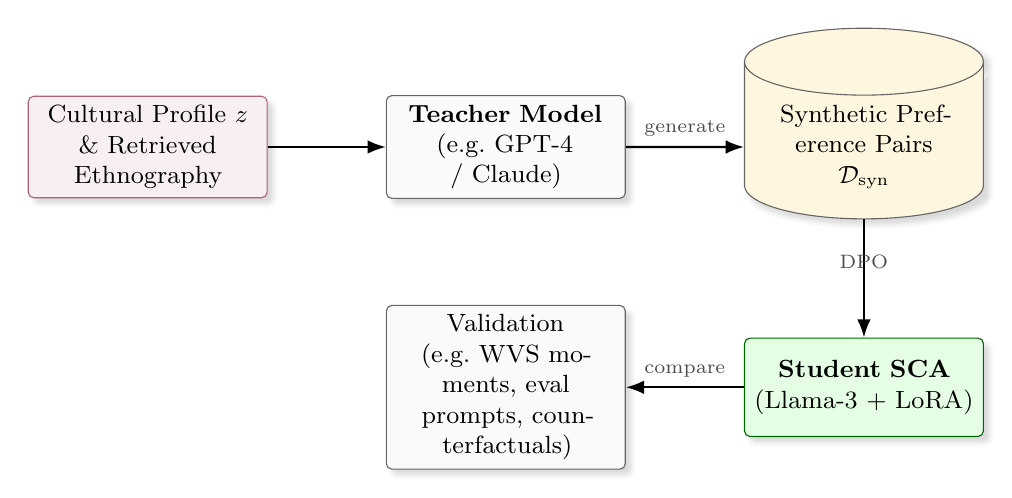
\begin{tikzpicture}[
    font=\small,
    node distance=1.5cm,
    >={Latex[length=3mm,width=2mm]},
    line/.style={draw, thick, -{Latex}},
    block/.style={
        rectangle, rounded corners=2pt,
        draw=black!60, fill=black!2,
        minimum height=1.25cm,
        text width=2.8cm, align=center,
        blur shadow={shadow blur steps=5, shadow blur extra rounding=1.5pt, shadow opacity=15}
    },
    data/.style={
        cylinder, shape border rotate=90, aspect=0.28,
        draw=black!60, fill=ASUGold!15,
        minimum height=1.25cm,
        text width=2.8cm, align=center,
        blur shadow={shadow blur steps=5, shadow blur extra rounding=1.5pt, shadow opacity=15}
    },
    emph/.style={fill=ASUMaroon!7, draw=ASUMaroon!70},
    ok/.style={fill=green!10, draw=green!40!black},
    note/.style={font=\scriptsize, text=black!70}
]
    % Nodes (horizontal)
    \node[block, emph] (profile) {Cultural Profile $z$\\ \& Retrieved Ethnography};
    \node[block] (teacher) [right=of profile] {\textbf{Teacher Model}\\(e.g.\ GPT-4 / Claude)};
    \node[data] (syn) [right=of teacher] {Synthetic Preference Pairs\\$\mathcal{D}_{\mathrm{syn}}$};
    \node[block, ok] (student) [below=of syn] {\textbf{Student SCA}\\(Llama-3 + LoRA)};
    \node[block] (eval) [left=of student] {Validation\\(e.g.\ WVS moments, eval prompts, counterfactuals)};

    % Arrows + labels
    \path[line] (profile) -- (teacher);
    \path[line] (teacher) -- node[note, above] {generate} (syn);
    \path[line] (syn) -- node[note, above] {DPO} (student);
    \path[line] (student) -- node[note, above] {compare} (eval);

\end{tikzpicture}
\caption{SCA 2.0 pipeline (high-level): culture-conditioned synthetic preference data from a teacher model is used to DPO-tune a student SCA; outputs are validated against external benchmarks (e.g., WVS).}
\label{fig:sca2-pipeline}
\end{figure}

\clearpage

%========================
% Appendix
%========================
\appendix
% --- Appendix Setup ---
\section*{Appendix: Mathematical Foundations and Derivations}

\noindent This appendix provides the formal derivations linking Reinforcement Learning from Human Feedback (RLHF) to Structural Microeconometrics, defines the state space for Cultural Agents, and details the synthetic data generation pipeline.

% --- SECTION A: PRELIMINARIES ---
\section{Preliminaries: The Language Model as a Policy}
\label{app:gemini}

\renewcommand{\thesubsection}{\Alph{section}.\arabic{subsection}}
\setcounter{section}{1} % Start A, B, C...

We define a Large Language Model (LLM) as a stochastic policy $\pi_\theta(y|x)$ parameterized by weights $\theta$.
\begin{itemize}
    \item \textbf{State space ($S$):} The set of all possible prompt histories $x$.
    \item \textbf{Action space ($A$):} The vocabulary set $V$ (tokens).
    \item \textbf{Trajectory ($y$):} A sequence of actions (completion) given context $x$.
\end{itemize}
The "Reference Policy" $\pi_{\text{ref}}$ denotes the pre-trained model (e.g., Llama-3), representing the prior distribution over language learned from the internet corpus.

% --- SECTION B: THEOREM 1 ---
\subsection{Theorem 1: The DPO-RUM Isomorphism}
\label{proof:dpo_rum}

We formally prove that the Direct Preference Optimization (DPO) objective is mathematically equivalent to the Maximum Likelihood Estimation (MLE) of a specific Random Utility Model (RUM).

\subsubsection{The Planner's Problem (RLHF)}
The alignment problem is formulated as a KL-constrained maximization of expected reward. The optimal policy $\pi^*$ solves:
\begin{equation}
    \max_{\pi} \mathbb{E}_{x \sim \mathcal{D}} \left[ \mathbb{E}_{y \sim \pi(\cdot|x)} [r^*(x, y)] - \beta D_{KL}(\pi(\cdot|x) || \pi_{\text{ref}}(\cdot|x)) \right]
    \label{eq:objective}
\end{equation}
where $r^*(x,y)$ is the latent utility function (unobserved) and $\beta > 0$ is the regularization parameter (temperature).

\textbf{Lemma 1 (Analytical Solution):} The closed-form solution to optimization problem (\ref{eq:objective}) is given by the tilted Gibbs distribution:
\begin{equation}
    \pi^*(y|x) = \frac{1}{Z(x)} \pi_{\text{ref}}(y|x) \exp\left( \frac{r^*(x, y)}{\beta} \right)
    \label{eq:optimal_policy}
\end{equation}
where $Z(x) = \sum_y \pi_{\text{ref}}(y|x) \exp(r^*(x, y)/\beta)$ is the partition function.

\begin{proof}
    This is a standard result in convex duality. The functional derivative of the Lagrangian with respect to $\pi$ yields the first-order condition $\log \pi(y|x) = \frac{1}{\beta} r^*(x,y) + \log \pi_{\text{ref}}(y|x) - 1 - \mu$, which rearranges to (\ref{eq:optimal_policy}).
\end{proof}

\subsubsection{The Inversion}
We invert Eq. (\ref{eq:optimal_policy}) to express the latent reward $r^*$ as a function of the optimal policy and the reference policy:
\begin{equation}
    r^*(x, y) = \beta \log \frac{\pi^*(y|x)}{\pi_{\text{ref}}(y|x)} + \beta \log Z(x)
    \label{eq:inverted_reward}
\end{equation}

\subsubsection{The Discrete Choice Model (Bradley-Terry)}
Assume the human evaluator's preferences follow a Bradley-Terry (Luce) model, which corresponds to a Random Utility Model with i.i.d. Gumbel error terms. The probability that completion $y_w$ is preferred to $y_l$ is:
\begin{equation}
    P(y_w \succ y_l | x) = \sigma(r^*(x, y_w) - r^*(x, y_l))
    \label{eq:bradley_terry}
\end{equation}
where $\sigma(u) = (1 + e^{-u})^{-1}$ is the logistic sigmoid function.

\subsubsection{The Substitution (The Isomorphism)}
Substitute the policy-defined reward (\ref{eq:inverted_reward}) into the preference model (\ref{eq:bradley_terry}). The difference in rewards is:
\begin{align*}
    r^*(x, y_w) - r^*(x, y_l) &= \left( \beta \log \frac{\pi^*(y_w|x)}{\pi_{\text{ref}}(y_w|x)} + \beta \log Z(x) \right) - \left( \beta \log \frac{\pi^*(y_l|x)}{\pi_{\text{ref}}(y_l|x)} + \beta \log Z(x) \right) \\
    &= \beta \log \frac{\pi^*(y_w|x)}{\pi_{\text{ref}}(y_w|x)} - \beta \log \frac{\pi^*(y_l|x)}{\pi_{\text{ref}}(y_l|x)}
\end{align*}
\textbf{Result:} The partition function term $\beta \log Z(x)$ cancels out. The likelihood of the preference data depends \textit{only} on the policies.

\subsubsection{The Structural Estimator}
The DPO loss function is the negative log-likelihood of this derived probability model:
\begin{equation}
    \mathcal{L}_{\text{DPO}}(\theta) = -\mathbb{E}_{(x, y_w, y_l) \sim \mathcal{D}} \left[ \log \sigma \left( \beta \log \frac{\pi_\theta(y_w|x)}{\pi_{\text{ref}}(y_w|x)} - \beta \log \frac{\pi_\theta(y_l|x)}{\pi_{\text{ref}}(y_l|x)} \right) \right]
\end{equation}
\textit{Economic Interpretation:} We are estimating the parameters of the policy function $\pi_\theta$ directly from revealed preference data, treating the log-ratio of the reference policy as a "price" or "base rate."

% --- SECTION C: CULTURAL STATE ---
\subsection{Modeling Culture: The State Vector $z$}
We reject ad-hoc definitions of culture in favor of the \textbf{Global Preferences Survey (GPS)} framework (Falk et al., QJE 2018). We define the cultural state vector $z \in [0,1]^6$ as:
\begin{equation}
    z = \begin{bmatrix} 
    \text{Time Preference} (\delta) \\ 
    \text{Risk Aversion} (\gamma) \\ 
    \text{Pos. Reciprocity} (\xi^+) \\ 
    \text{Neg. Reciprocity} (\xi^-) \\ 
    \text{Altruism} (\alpha) \\ 
    \text{Trust} (\tau)
    \end{bmatrix}
\end{equation}
These parameters map directly to the primitives of a standard utility function $U(c_t; z)$. An SCA is defined as a policy $\pi(\cdot|s; z)$ conditioned on this vector.

% --- SECTION D: ALGORITHM ---
\subsection{Algorithm 1: Synthetic Ethnography (Teacher-Student Distillation)}\label{sec:algo}
To calibrate SCAs for populations with scarce digital traces (e.g., non-WEIRD populations), we employ a two-step distillation process.

\begin{figure}[htbp]
    \centering
    \begin{adjustbox}{max width=\textwidth}
        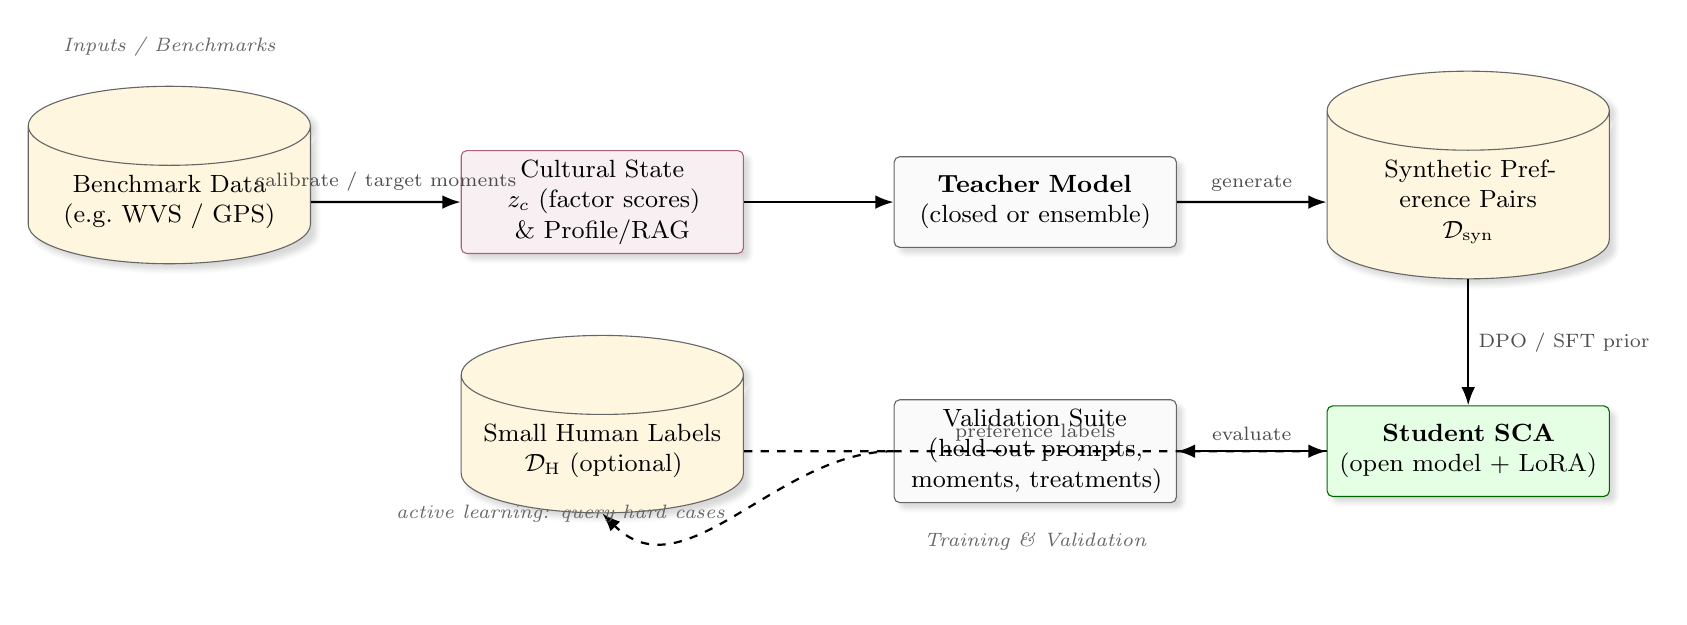
\begin{tikzpicture}[
            font=\small,
            node distance=1.6cm and 1.9cm,
            >={Latex[length=3mm,width=2mm]},
            line/.style={draw, thick, -{Latex}},
            dashedline/.style={draw, thick, -{Latex}, dashed},
            block/.style={
                rectangle, rounded corners=2pt,
                draw=black!60, fill=black!2,
                minimum height=1.15cm,
                text width=3.35cm, align=center,
                blur shadow={shadow blur steps=5, shadow blur extra rounding=1.5pt, shadow opacity=15}
            },
            data/.style={
                cylinder, shape border rotate=90, aspect=0.28,
                draw=black!60, fill=ASUGold!15,
                minimum height=1.15cm,
                text width=3.35cm, align=center,
                blur shadow={shadow blur steps=5, shadow blur extra rounding=1.5pt, shadow opacity=15}
            },
            emph/.style={fill=ASUMaroon!7, draw=ASUMaroon!70},
            ok/.style={fill=green!10, draw=green!40!black},
            note/.style={font=\scriptsize, text=black!70},
            smallnote/.style={font=\scriptsize\itshape, text=black!60}
        ]
        
        % --- Top row: inputs / benchmarks ---
        \node[data] (wvs) {Benchmark Data\\(e.g.\ WVS / GPS)};
        \node[block, emph] (state) [right=of wvs] {Cultural State\\$z_c$ (factor scores)\\\& Profile/RAG};
        \node[block] (teacher) [right=of state] {\textbf{Teacher Model}\\(closed or ensemble)};
        \node[data] (syn) [right=of teacher] {Synthetic Preference Pairs\\$\mathcal{D}_{\mathrm{syn}}$};
        
        % --- Bottom row: training / evaluation ---
        \node[block, ok] (student) [below=1.6cm of syn] {\textbf{Student SCA}\\(open model + LoRA)};
        \node[block] (eval) [left=of student] {Validation Suite\\(held-out prompts,\\moments, treatments)};
        \node[data] (human) [left=of eval] {Small Human Labels\\$\mathcal{D}_{\mathrm{H}}$ (optional)};
        
        % --- Flows ---
        \path[line] (wvs) -- node[note, above] {calibrate / target moments} (state);
        \path[line] (state) -- (teacher);
        \path[line] (teacher) -- node[note, above] {generate} (syn);
        \path[line] (syn) -- node[note, right] {DPO / SFT prior} (student);
        
        \path[line] (student) -- node[note, above] {evaluate} (eval);
        
        % --- Optional correction loop (dashed) ---
        \path[dashedline] (human) -- node[note, above] {preference labels} (student);
        \path[dashedline] (eval.west) to[out=180,in=-45] node[smallnote, left] {active learning: query hard cases} (human.south);
        
        % --- Subtle grouping labels ---
        \node[smallnote, above=0.25cm of wvs] {Inputs / Benchmarks};
        \node[smallnote, below=0.25cm of eval] {Training \& Validation};
        
        \end{tikzpicture}
    \end{adjustbox}
    \caption{SCA 2.0 pipeline with explicit separation between (i) benchmark data used to calibrate cultural state and evaluation targets, (ii) synthetic preference generation, and (iii) student tuning with an optional human-correction loop.}
    \label{fig:sca2-pipeline-extended}
\end{figure}

\begin{enumerate}
    \item \textbf{Teacher Phase (Data Generation):}
    \begin{itemize}
        \item \textbf{Input:} Cultural Profile $P_c$ (Ethnographic text + GPS moments).
        \item \textbf{Model:} Large frontier instruction model.
        \item \textbf{Action:} Generate $N=10,000$ synthetic survey responses and economic decisions.
        \item \textbf{Output:} Synthetic Dataset $\mathcal{D}_{\text{syn}} = \{(x, y_w, y_l)\}$.
    \end{itemize}
    
    \item \textbf{Student Phase (Structural Estimation):}
    \begin{itemize}
        \item \textbf{Input:} Base Model $\pi_{\text{ref}}$ (Llama-3-8B).
        \item \textbf{Objective:} Minimize $\mathcal{L}_{\text{DPO}}(\theta)$ on $\mathcal{D}_{\text{syn}}$.
        \item \textbf{Result:} A calibrated SCA $\pi_{\text{SCA}}$ that internalizes the cultural priors into its weights.
    \end{itemize}
\end{enumerate}

\subsection{Remark on Reasoning (Group Relative Policy Optimization)}
Recent advances, such as DeepSeek-R1's GRPO, extend this framework to sequential reasoning. GRPO replaces the pairwise loss with a group-based advantage estimator:
$$ A_i = \frac{r_i - \text{mean}(\{r_1, \dots, r_G\})}{\text{std}(\{r_1, \dots, r_G\})} $$
This can be interpreted as a non-parametric approximation of the Value Function $V(s)$, allowing the SCA to "reason" about cultural norms over multiple steps without a trained critic network.

\section{Random utility, logit, and Bradley--Terry}\label{app:rum}

This appendix is written as a self-contained primer for readers with first-year PhD economics probability and optimization.

\subsection{Notation and measurability (minimal)}
Let $(\Omega,\mathcal{F},\mathcal{P})$ be a probability space. For each context $x\in\mathcal{X}$, let $\mathcal{Y}(x)$ denote the set of feasible responses
(e.g., all token sequences up to length $T$, or a finite candidate set produced by sampling).
A (stochastic) policy $\pi(\cdot\mid x)$ is a probability measure on $\mathcal{Y}(x)$.
When $\mathcal{Y}(x)$ is countable, sums are literal; otherwise interpret $\sum_y$ as $\int \dd y$.

\subsection{Bradley--Terry as logistic regression on utility differences}
\begin{definition}[Bradley--Terry model]
Given a real-valued score $r(x,y)$, the BT model specifies paired-comparison probabilities as
\[
\mathcal{P}(y_1 \succ y_2 \mid x)
=
\frac{\exp(r(x,y_1))}{\exp(r(x,y_1))+\exp(r(x,y_2))}
=
\sigmoid(r(x,y_1)-r(x,y_2)).
\]
\end{definition}

Given labeled pairs $\{(x_i,y_i^{(w)},y_i^{(\ell)})\}$, the BT log-likelihood is
\begin{equation}\label{eq:bt-ll}
\ell(r;\mathcal{D})
=
\sum_{i=1}^N \log \sigmoid\!\Big(r(x_i,y_i^{(w)})-r(x_i,y_i^{(\ell)})\Big).
\end{equation}
\textbf{Identification.} For each fixed $x$, $r(x,\cdot)$ is identified only up to an additive constant $c(x)$,
since differences $r(x,y_1)-r(x,y_2)$ are invariant to $r(x,\cdot)\mapsto r(x,\cdot)+c(x)$.

\subsection{Microfoundation: random utility with Type-I EV shocks}
Let latent utility be
\[
U(x,y)=r(x,y)+\varepsilon_y,
\]
with $(\varepsilon_y)_{y\in\mathcal{Y}(x)}$ i.i.d. Type-I extreme value (Gumbel).
Then for two alternatives $y_1,y_2$,
\[
\mathcal{P}(y_1 \succ y_2 \mid x)
=
\mathcal{P}\big(U(x,y_1)\ge U(x,y_2)\big)
=
\sigmoid\!\big(r(x,y_1)-r(x,y_2)\big).
\]
This yields BT/logit. For more than two alternatives, the same assumption yields multinomial logit with the IIA property.

\begin{remark}[Why Gumbel matters]
The Gumbel assumption is the reason log-sum-exp and softmax appear everywhere:
\[
\E\left[\max_{y}\{r(x,y)+\varepsilon_y\}\right]
=
\beta \log \sum_y \exp(r(x,y)/\beta) + \text{const}.
\]
This is the ``inclusive value'' interpretation in discrete choice and it reappears as the value function in soft RL (Appendix \ref{app:softbellman}).
\end{remark}

\section{KL-regularized optimization and the softmax policy}\label{app:kl}

This section proves the closed-form optimizer used in RLHF-KL objectives and establishes the key log-ratio identity.

\subsection{Problem}
Fix a context $x$ and consider
\begin{equation}\label{eq:inner}
\max_{\pi(\cdot\mid x)}\;
\sum_{y}\pi(y\mid x)\,r(x,y)
-
\beta\sum_{y}\pi(y\mid x)\log\frac{\pi(y\mid x)}{\refpol(y\mid x)}
\quad\text{s.t.}\quad
\sum_y \pi(y\mid x)=1,\;\pi\ge 0.
\end{equation}
Assume $r(x,\cdot)$ is bounded above (or integrable) and $\refpol(y\mid x)>0$ on the support of interest.

\subsection{Existence and uniqueness}
\begin{lemma}[Concavity and existence]
The objective in \eqref{eq:inner} is strictly concave in $\pi(\cdot\mid x)$ and attains a unique maximizer $\pi^\star(\cdot\mid x)$.
\end{lemma}
\begin{proof}
Strict concavity follows because $-\KL(\pi\|\refpol)$ is strictly concave in $\pi$ on the simplex when $\refpol$ is strictly positive on support.
The feasible set is compact (simplex) and the objective is upper semicontinuous under mild integrability; hence a maximizer exists, and strict concavity yields uniqueness.
\end{proof}

\subsection{Closed form via Lagrange multipliers}
\begin{lemma}[Softmax around the reference]\label{lem:softmax}
The unique optimizer of \eqref{eq:inner} satisfies
\[
\pi^\star(y\mid x)
=
\frac{\refpol(y\mid x)\exp(r(x,y)/\beta)}{Z(x)},
\qquad
Z(x)=\sum_{y'} \refpol(y'\mid x)\exp(r(x,y')/\beta).
\]
\end{lemma}
\begin{proof}
Form the Lagrangian
\[
\mathcal{L}(\pi,\lambda)
=
\sum_y \pi(y\mid x)r(x,y)
-
\beta\sum_y \pi(y\mid x)\log\frac{\pi(y\mid x)}{\refpol(y\mid x)}
+
\lambda\Big(\sum_y \pi(y\mid x)-1\Big).
\]
For any $y$ with $\pi(y\mid x)>0$, the stationarity condition is
\[
0=\frac{\partial\mathcal{L}}{\partial \pi(y\mid x)}
=
r(x,y) -\beta\Big(\log\frac{\pi(y\mid x)}{\refpol(y\mid x)}+1\Big)+\lambda.
\]
Rearrange:
\[
\log\frac{\pi(y\mid x)}{\refpol(y\mid x)}=\frac{r(x,y)+\lambda-\beta}{\beta}.
\]
Exponentiate and normalize to satisfy $\sum_y \pi(y\mid x)=1$, yielding the stated form with a partition function $Z(x)$.
\end{proof}

\subsection{Key inversion: rewards as log probability ratios}
\begin{corollary}[Log-ratio identity]\label{cor:logratio}
Let $\pi^\star$ satisfy Lemma \ref{lem:softmax}. Then for any $y$,
\[
r(x,y)
=
\beta\log\frac{\pi^\star(y\mid x)}{\refpol(y\mid x)} + \beta\log Z(x).
\]
Hence for any $y_1,y_2$,
\[
r(x,y_1)-r(x,y_2)
=
\beta\left[
\log\frac{\pi^\star(y_1\mid x)}{\refpol(y_1\mid x)}-\log\frac{\pi^\star(y_2\mid x)}{\refpol(y_2\mid x)}
\right].
\]
\end{corollary}
\begin{proof}
Take logs of Lemma \ref{lem:softmax} and rearrange; the $Z(x)$ term cancels in differences.
\end{proof}

\section{Deriving the DPO objective from BT + KL-regularized optimality}\label{app:dpo}

This section gives the derivation in referee-proof detail.

\subsection{Assumptions}
\begin{enumerate}[leftmargin=1.2cm, itemsep=0.2em]
\item \textbf{BT preference model.} Human labels are generated by \eqref{eq:BT} with some latent reward $r^\star(x,y)$.
\item \textbf{KL-optimality.} The (unknown) optimal policy $\pi^\star$ for reward $r^\star$ satisfies Lemma \ref{lem:softmax} with reference $\refpol$ and temperature $\beta$.
\end{enumerate}

\subsection{From BT to log-ratio scores}
Start from BT:
\[
\mathcal{P}(y_w \succ y_\ell\mid x)=\sigmoid(r^\star(x,y_w)-r^\star(x,y_\ell)).
\]
By Corollary \ref{cor:logratio},
\[
r^\star(x,y_w)-r^\star(x,y_\ell)
=
\beta\left[
\log\frac{\pi^\star(y_w\mid x)}{\refpol(y_w\mid x)}
-
\log\frac{\pi^\star(y_\ell\mid x)}{\refpol(y_\ell\mid x)}
\right].
\]
Thus the BT probability can be written as
\begin{equation}\label{eq:bt-logratio}
\mathcal{P}(y_w \succ y_\ell\mid x)=
\sigmoid\!\left(
\beta\left[
\log\frac{\pi^\star(y_w\mid x)}{\refpol(y_w\mid x)}
-
\log\frac{\pi^\star(y_\ell\mid x)}{\refpol(y_\ell\mid x)}
\right]\right).
\end{equation}

\subsection{Likelihood for a parametric policy}
We do not observe $\pi^\star$. We posit a parametric family $\{\pi_\theta\}$ and fit it by maximum likelihood under the model \eqref{eq:bt-logratio}.
Given $\mathcal{D}$,
\[
\ell(\theta;\mathcal{D})
=
\sum_{i=1}^N
\log
\sigmoid\!\left(
\beta\left[
\log\frac{\pi_\theta(y_i^{(w)}\mid x_i)}{\refpol(y_i^{(w)}\mid x_i)}
-
\log\frac{\pi_\theta(y_i^{(\ell)}\mid x_i)}{\refpol(y_i^{(\ell)}\mid x_i)}
\right]\right).
\]
Define the \emph{DPO loss} as $\mathcal{L}_{\mathrm{DPO}}(\theta)=-\ell(\theta;\mathcal{D})$.
This is the standard objective used in DPO implementations.

\subsection{Interpretation: what is being estimated?}
It is tempting to say we are ``estimating $r^\star$,'' but DPO avoids an explicit reward model.
Instead, it estimates the \emph{policy} whose log-ratio scores explain preference labels under BT.
Reward differences are implicitly represented by policy log-ratio differences.

\begin{remark}[Temperature / scale]
The parameter $\beta$ is a scale normalization that controls how sharply preferences respond to score differences.
In structural choice models, it plays the role of a shock scale (variance) parameter.
In RLHF, it controls how far the learned policy can move from $\refpol$ before KL costs dominate.
\end{remark}

\begin{remark}[Misspecification]
If BT is misspecified (e.g., preferences violate IIA-like properties across candidate sets, raters are inconsistent, context effects),
DPO remains a valid M-estimator for the best-fitting logit model, but the interpretation of $r^\star$ as ``true utility'' becomes approximate.
\end{remark}

\section{Soft Bellman equations and process supervision}\label{app:softbellman}

This section extends the one-step analysis to sequential decision-making over tokens or reasoning steps.

\subsection{MDP setup}
Let $(\mathcal{S},\mathcal{A},P,r,\gamma)$ be an MDP:
\begin{itemize}
    \item $s\in\mathcal{S}$ is a state (e.g., prompt + partial transcript),
    \item $a\in\mathcal{A}(s)$ an action (token),
    \item $P(\cdot\mid s,a)$ a transition kernel,
    \item $r(s,a)$ a bounded reward, and $\gamma\in(0,1)$ a discount factor.
\end{itemize}
Let $\refpol(a\mid s)$ be a reference policy.

Consider the maximum-entropy / KL-regularized objective:
\begin{equation}\label{eq:entrl}
\max_{\pi}\;
\E^\pi\left[\sum_{t\ge 0}\gamma^t \Big(r(s_t,a_t) - \beta\log\frac{\pi(a_t\mid s_t)}{\refpol(a_t\mid s_t)}\Big)\right].
\end{equation}

\subsection{Soft Bellman operator}
Define the soft Q-function:
\[
Q(s,a)= r(s,a) + \gamma \E[V(s')\mid s,a].
\]
Then the optimal value satisfies
\begin{equation}\label{eq:softV}
V^\star(s)
=
\beta\log\sum_{a}\refpol(a\mid s)\exp\Big(\tfrac{1}{\beta}Q^\star(s,a)\Big),
\end{equation}
and the optimal policy is
\begin{equation}\label{eq:softpi}
\pi^\star(a\mid s)
=
\frac{\refpol(a\mid s)\exp(\tfrac{1}{\beta}Q^\star(s,a))}{\sum_{a'}\refpol(a'\mid s)\exp(\tfrac{1}{\beta}Q^\star(s,a'))}.
\end{equation}

\begin{theorem}[Contraction and existence]\label{thm:contraction}
Assume $|r(s,a)|\le R_{\max}<\infty$ and $\gamma\in(0,1)$. Define the soft Bellman operator $(\mathcal{T}V)(s)$ by
\[
(\mathcal{T}V)(s)
=
\beta\log\sum_{a}\refpol(a\mid s)\exp\Big(\tfrac{1}{\beta}\big[r(s,a)+\gamma \E[V(s')\mid s,a]\big]\Big).
\]
Then $\mathcal{T}$ is a contraction on bounded functions under the sup norm, hence has a unique fixed point $V^\star$.
\end{theorem}
\begin{proof}
Use the standard DP argument plus Lipschitzness of log-sum-exp: for any vectors $u,v$, $|\mathrm{LSE}(u)-\mathrm{LSE}(v)|\le \|u-v\|_\infty$.
Then $|(\mathcal{T}V)(s)-(\mathcal{T}W)(s)|\le \gamma\|V-W\|_\infty$. Take sup over $s$.
\end{proof}

\subsection{Graphical intuition: log-sum-exp as ``soft max''}
For scalars $z_1,z_2$,
\[
\beta\log\big(e^{z_1/\beta}+e^{z_2/\beta}\big)
\approx \max\{z_1,z_2\} \quad\text{as }\beta\to 0,
\]
and becomes smoother as $\beta$ grows. This is why entropy regularization makes optimization stable and why the value is an ``inclusive value.''

\begin{center}
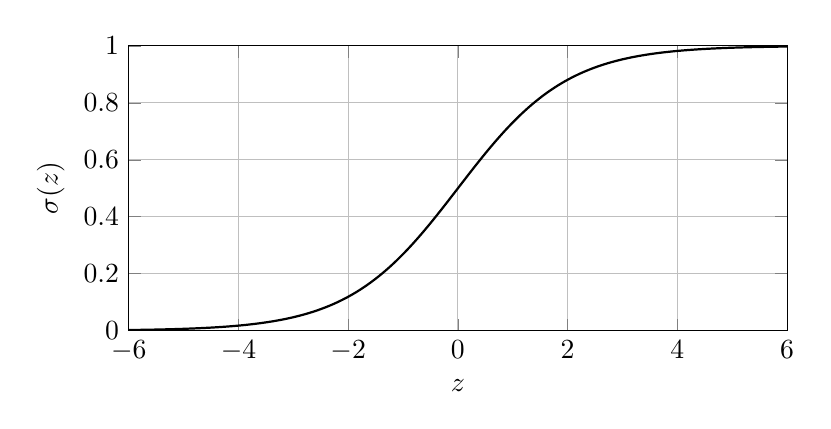
\begin{tikzpicture}
\begin{axis}[
  width=0.82\textwidth,
  height=5.2cm,
  xlabel={$z$},
  ylabel={$\sigmoid(z)$},
  grid=major,
  xmin=-6, xmax=6,
  ymin=0, ymax=1,
  ticks=both
]
\addplot[domain=-6:6,samples=300,thick] {1/(1+exp(-x))};
\end{axis}
\end{tikzpicture}
\end{center}

\noindent The logistic function appears in BT probabilities and, via log-ratio scores, in DPO training.

\section{Structural dynamic discrete choice: the econometric mirror}\label{app:ddc}

In structural dynamic discrete choice (DDC) models with Type-I EV shocks, the probability of choosing action $a$ in state $s$ takes a logit form in choice-specific value functions.
Hotz--Miller (1993) shows that \emph{conditional choice probabilities} (CCPs) can be inverted to recover differences in choice-specific value functions up to constants.

\subsection{Why this matters here}
The DPO derivation uses the same algebraic structure:
\begin{itemize}[leftmargin=1.2cm, itemsep=0.2em]
\item DDC: estimate CCPs from data, invert to get value differences, avoid repeated solution of the DP.
\item DPO: parameterize $\pi_\theta$, use BT likelihood on preference pairs, and via log-ratio identities interpret score differences as reward/value differences (relative to $\refpol$), avoiding explicit reward-model estimation.
\end{itemize}

This provides an economist-native narrative: DPO is an inversion-based estimator for a regularized discrete-choice control problem.

\section{Worked examples and diagnostics}\label{app:examples}

\subsection{Example 1: Finite candidate set}
Let $\mathcal{Y}(x)=\{y^{(1)},\dots,y^{(K)}\}$ be a finite set of candidate responses produced by sampling.
Then BT probabilities are well-defined on the finite set and the partition function $Z(x)$ in \eqref{eq:softmax} is a finite sum.
This is the cleanest setting for proofs and intuition.

\subsection{Example 2: Continuous outputs (measure-theoretic note)}
If $\mathcal{Y}(x)$ is uncountable (all token sequences), replace sums with integrals w.r.t. a base measure.
In practice, both preference labeling and DPO training operate on \emph{finite sampled sets} of responses,
so the finite-candidate analysis captures the implemented estimand.

\subsection{Diagnostic: invariances and failure modes}
\begin{enumerate}[leftmargin=1.2cm, itemsep=0.2em]
\item \textbf{Additive constants.} $r(x,\cdot)$ is identified up to $c(x)$. DPO implicitly absorbs this into $Z(x)$.
\item \textbf{Support mismatch.} If $\refpol(y\mid x)=0$ but $\pi_\theta(y\mid x)>0$, log ratios blow up. In practice, models share support.
\item \textbf{Label noise / context effects.} BT assumes a single latent $r^\star$ with logistic noise. If preferences depend on the presented pair set,
or are non-transitive, BT is misspecified; DPO remains an M-estimator but the ``utility'' interpretation weakens.
\end{enumerate}

\subsection{A small ``dictionary'' for later specialization}
\begin{center}
\begin{tabular}{@{}ll@{}}
\toprule
Structural economics & Preference-based fine-tuning \\
\midrule
Context / environment $x$ & Prompt / task $x$ \\
Alternative $y$ & Candidate completion $y$ \\
Utility $u(x,y)$ & Reward / score $r(x,y)$ \\
Random utility shocks & Rater noise / preference randomness \\
Logit/BT likelihood & Pairwise preference loss (DPO) \\
CCP inversion (Hotz--Miller) & Log-ratio identity (Cor. \ref{cor:logratio}) \\
Entropy / info cost & KL to reference policy \\
\bottomrule
\end{tabular}
\end{center}

\noindent This dictionary is the backbone for specializing to cultural alignment later: ``culture'' becomes either a parameter in $r(x,y;c)$ or a shifter of the state distribution.


\clearpage
\printbibliography
\end{document}